\chapter{Hajautustaulu}

\index{hajautustaulu}

\emph{Hajautustaulu} (\emph{hash table}) on tietorakenne,
joka tarjoaa tehokkaat operaatiot alkion lisäämiseen,
hakemiseen ja poistamiseen.
Voimme toteuttaa hajautustaulun avulla \emph{joukon},
jossa on kokoelma alkioita, sekä sen laajennoksena
\emph{hakemiston}, jossa alkiot ovat avain-arvo-pareja.

Yksi tapa ajatella hajautusta on, että yleistämme taulukon ideaa:
taulukossa indeksit ovat aina 0, 1, 2, jne., mutta hajautustaulussa
voimme käyttää indeksien sijasta vaikkapa merkkijonoja.
Tämä onnistuu käyttämällä hajautusfunktiota,
joka muuttaa muun tyyppisen alkion indeksiksi,
jotta löydämme sille paikan taulukosta.

\section{Hajautustaulun toteutus}

\index{hajautusfunktio}
\index{hajautusarvo}

Hajautustaulun perustana on \emph{hajautusfunktio}
(\emph{hash function}) $f(x)$,
joka antaa \emph{hajautusarvon} (\emph{hash value})
mille tahansa alkiolle $x$.
Hajautusarvo on kokonaisluku väliltä $0,1,\dots,N-1$,
missä $N$ on hajautustaulun koko.
Hajautusarvo määrää, mihin hajautustaulun kohtaan
alkio tallennetaan.

Tarkastellaan esimerkkinä hajautusfunktiota $f(x)=x \bmod N$,
missä $x$ on kokonaisluku.
Tämä hajautusfunktio antaa hajautusarvoksi luvun $x$
jakojäännöksen $N$:llä.
Esimerkiksi jos $N=10$ ja tallennamme hajautustauluun luvun 14,
saamme sen hajautusarvoksi $f(14)=4$.
Tämä tarkoittaa, että luvun paikka hajautustaulussa on kohdassa 4.
Vastaavasti $f(21)=1$, eli luvun 21 paikka hajautustaulussa on
kohdassa 1.

\index{törmäys}

Yleensä hajautustaulun koko $N$ on selvästi pienempi kuin
mahdollisten alkioiden määrä ja
hajautuksessa voi tapahtua \emph{törmäys} (\emph{collision})
eli kahdelle alkiolle tulee sama hajautusarvo.
Esimerkiksi $f(14)=f(24)=4$ eli luvut 14 ja 24 kuuluvat
samaan paikkaan hajautustaulussa.
Tämän vuoksi hajautustaulun toteutuksessa täytyy päättää,
miten tör\-mäykset käsitellään.
Kaksi tavallista tapaa tähän ovat ketjuhajautus sekä avoin hajautus.

\subsection{Ketjuhajautus}

\begin{figure}
\center
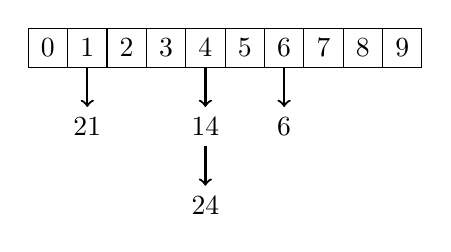
\begin{tikzpicture}[scale=0.5]
\draw (0,0) grid (10,1);
\foreach \x in {0,1,...,9} \node at (0.5+\x,0.5) {\x};
\draw[->,thick] (1.5,0) -- (1.5,-1);
\draw[->,thick] (6.5,0) -- (6.5,-1);
\draw[->,thick] (4.5,0) -- (4.5,-1);
\draw[->,thick] (4.5,-2) -- (4.5,-3);
\node at (1.5,-1.5) {$21$};
\node at (6.5,-1.5) {$6$};
\node at (4.5,-1.5) {$14$};
\node at (4.5,-3.5) {$24$};
\end{tikzpicture}
\caption{Ketjuhajautusta käyttävä hajautustaulu, joka vastaa joukkoa $\{6,14,21,24\}$.
Hajautusfunktiona on $f(x)=x \bmod N$.}
\label{fig:hajtau}
\end{figure}

\index{ketjuhajautus}

\emph{Ketjuhajautus} (\emph{chaining})
on hajautustaulun toteutustapa, jossa jokainen hajautustaulun kohta
sisältää listan alkioista,
joilla on kyseinen hajautusarvo.
Tällöin mahdolliset alkioiden törmäykset eivät haittaa,
koska listoissa voi olla mikä tahansa määrä alkioita.

Kuvassa \ref{fig:hajtau} on esimerkkinä
ketjuhajautusta käyttävä hajautustaulu,
johon on tallennettu joukko $\{6,14,21,24\}$
käyttäen hajautusfunktiota $f(x)=x \bmod N$.
Kohdassa 1 on alkio 21, kohdassa 4 on alkiot 14 ja 24
ja kohdassa 6 on alkio 6.
Muissa kohdissa olevat listat ovat vielä tyhjiä.

Kun haluamme tarkastaa, onko joukossa alkiota $x$,
laskemme ensin sen hajautusarvon $f(x)$.
Tämän jälkeen käymme läpi kaikki kohdan $f(x)$
listassa olevat alkiot ja tarkastamme,
onko jokin niistä alkio $x$.
Vastaavasti kun haluamme lisätä alkion $x$ joukkoon
tai poistaa alkion $x$ joukosta,
teemme muutoksen kohdassa $f(x)$ olevaan listaan.

\begin{figure}
\center
\begin{tikzpicture}[scale=0.5]
\begin{scope}
\draw (0,0) grid (10,1);
\foreach \x in {0,1,...,9} \node at (0.5+\x,0.5) {\x};
\draw[->,thick] (1.5,0) -- (1.5,-1);
\draw[->,thick] (4.5,0) -- (4.5,-1);
\draw[->,thick] (5.5,0) -- (5.5,-1);
\draw[->,thick] (8.5,0) -- (8.5,-1);
\node at (1.5,-1.5) {$14$};
\node at (4.5,-1.5) {$21$};
\node at (5.5,-1.5) {$6$};
\node at (8.5,-1.5) {$24$};
\end{scope}
\begin{scope}[xshift=12cm]
\draw (0,0) grid (10,1);
\foreach \x in {0,1,...,9} \node at (0.5+\x,0.5) {\x};
\draw[->,thick] (3.5,0) -- (3.5,-1);
\draw[->,thick] (3.5,-2) -- (3.5,-3);
\draw[->,thick] (3.5,-4) -- (3.5,-5);
\draw[->,thick] (3.5,-6) -- (3.5,-7);
\node at (3.5,-1.5) {$21$};
\node at (3.5,-3.5) {$14$};
\node at (3.5,-5.5) {$24$};
\node at (3.5,-7.5) {$6$};
\end{scope}
\end{tikzpicture}
\caption{Kaksi hajautustaulua joukolle $\{6,14,21,24\}$.
Vasen tilanne on paras mahdollinen, oikea tilanne taas
huonoin mahdollinen.}
\label{fig:hajjak}
\end{figure}

Ketjuhajautuksessa
hajautustaulun operaatioiden aikavaativuus on $O(m)$,
missä $m$ on listan alkioiden määrä.
Hajautustaulu toimii siis tehokkaasti, jos
siinä olevat listat ovat lyhyitä.
Tämä toteutuu, jos käytetty hajautusfunktio sijoittaa
alkioita tasaisesti hajautustaulun eri puolille.
Kuvassa \ref{fig:hajjak} on kaksi ääriesimerkkiä
hajautuksen onnistumisesta erilaisilla hajautusfunktioilla.
Vasemmassa hajautustaulussa jokainen alkio on eri listassa,
mikä on paras mahdollinen tilanne.
Oikeassa hajautustaulussa kaikki alkiot ovat puolestaan samassa listassa,
mikä on huonoin mahdollinen tilanne.

\subsection{Avoin hajautus}

\index{avoin hajautus}

Toinen tapa toteuttaa hajautustaulu on \emph{avoin hajautus}
(\emph{open addressing}),
jossa alkiot tallennetaan suoraan hajautustauluun listojen sijasta.
Kuitenkin jos alkio kuuluisi paikkaan, jossa on jo valmiina
jokin toinen alkio, sille valitaan toinen paikka jonkin säännön perusteella.

\index{kokeilufunktio}
\index{lineaarinen kokeilu}

Avoimessa hajautuksessa alkion paikkaa hajautustaulussa etsitään
\emph{kokeilufunktiolla} (\emph{probe function})
$h(x,i)$, jossa $x$ on alkio ja $i$ ilmaisee, montako kertaa
sille on yritetty etsiä paikkaa.
Tarkastelemme seuraavaksi yksinkertaista kokeilufunktiota
\[ h(x,i) = (f(x)+i) \bmod N,\]
mikä tarkoittaa, että alkiolle etsitään paikkaa sen
hajautusarvon $f(x)$ antamasta kohdasta lähtien kulkemalla taulukossa oikealle,
kunnes vapaa paikka löytyy.
Tämän menetelmän nimi on \emph{lineaarinen kokeilu}
(\emph{linear probing}).

Kuvassa \ref{fig:hajavo} näkyy joukon $\{6,14,21,24\}$
sijoittuminen hajautustauluun
käyttäen hajautusfunktiota $f(x)=x \bmod N$ ja lineaarista kokeilua.
Tässä alkio 14 on lisätty ennen alkiota 24,
minkä vuoksi alkio 14 on sen hajautusarvon mukaisessa kohdassa 4
mutta alkio 24 on kohdassa 5, koska kohta 4 oli jo varattu.
Kuvassa \ref{fig:hajav2} mukaan lisätään vielä alkio 44,
jolla on myös hajautusarvo 4.
Koska kohdissa 4, 5 ja 6 on jo alkio, alkion 44 kohdaksi tulee 7.
Alkio voi sijoittua siis kauaskin hajautusarvon määräämästä kohdasta,
jos hajautustaulussa on täyttä.

\begin{figure}
\center
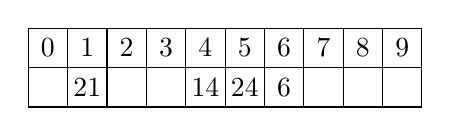
\begin{tikzpicture}[scale=0.5]
\draw (0,-1) grid (10,1);
\foreach \x in {0,1,...,9} \node at (0.5+\x,0.5) {\x};
\node at (1.5,-0.5) {$21$};
\node at (6.5,-0.5) {$6$};
\node at (4.5,-0.5) {$14$};
\node at (5.5,-0.5) {$24$};
\end{tikzpicture}
\caption{Avointa hajautusta käyttävä hajautustaulu, joka vastaa joukkoa $\{6,14,21,24\}$.
Hajautusfunktiona on $f(x)=x \bmod N$.}
\label{fig:hajavo}
\end{figure}

\begin{figure}
\center
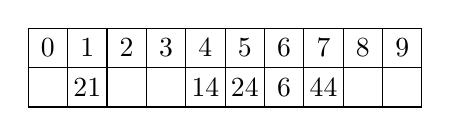
\begin{tikzpicture}[scale=0.5]
\draw (0,-1) grid (10,1);
\foreach \x in {0,1,...,9} \node at (0.5+\x,0.5) {\x};
\node at (1.5,-0.5) {$21$};
\node at (6.5,-0.5) {$6$};
\node at (4.5,-0.5) {$14$};
\node at (5.5,-0.5) {$24$};
\node at (7.5,-0.5) {$44$};
\end{tikzpicture}
\caption{Hajautustauluun lisätään vielä alkio 44, jonka hajautusarvo on 4.
Sille löytyy paikka vasta kohdasta 7.}
\label{fig:hajav2}
\end{figure}

Kun haluamme löytää alkion $x$ hajautustaulusta avointa hajautusta käyt\-täen,
aloitamme kohdasta $f(x)$ ja tutkimme sitten kohtia kokeilufunktion mukaisesti,
kunnes joko löydämme alkion tai tulemme tyhjään kohtaan, jolloin voimme päätellä,
että hajautustaulussa ei ole alkiota.
Esimerkiksi kun haluamme löytää kuvan \ref{fig:hajav2} hajautustaulusta
alkion 44, aloitamme kohdasta $f(44)=4$ ja kuljemme eteenpäin kohtaan 7 asti.

Alkion poistaminen aiheuttaa hieman ongelmia avoimessa hajautuksessa,
koska jos vain merkitsemme alkion kohdan tyhjäksi, tämä voi häiritä tulevia hakuja.
Esimerkiksi jos poistaisimme kuvan \ref{fig:hajav2} hajautustaulusta alkion 6
merkitsemällä kohdan 6 tyhjäksi, emme enää löytäisi alkiota 44,
koska haku pysähtyisi tyhjään kohtaan 6.
Kuitenkin voimme kiertää ongelman käyttämällä jotain erikoismerkkiä
poistetulle alkiolle. Kuvassa \ref{fig:hajav3} poistetun alkion merkkinä on X,
joka tarkoittaa, että kyseinen kohta on tyhjä mutta siinä on ollut alkio.
Niinpä alkion 44 haku ei pääty tähän kohtaan,
vaikka siihen voi myös sijoittaa uuden alkion myöhemmin.

\begin{figure}
\center
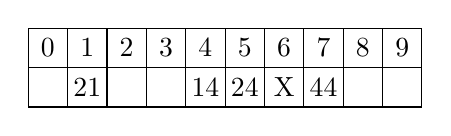
\begin{tikzpicture}[scale=0.5]
\draw (0,-1) grid (10,1);
\foreach \x in {0,1,...,9} \node at (0.5+\x,0.5) {\x};
\node at (1.5,-0.5) {$21$};
\node at (6.5,-0.5) {X};
\node at (4.5,-0.5) {$14$};
\node at (5.5,-0.5) {$24$};
\node at (7.5,-0.5) {$44$};
\end{tikzpicture}
\caption{Hajautustaulusta on poistettu alkio 6, jonka tilalla on merkki X.
Tämän ansiosta alkion 44 haku ei pysähdy kohtaan 6.}
\label{fig:hajav3}
\end{figure}

Avoimen hajautuksen tehokkuus riippuu sekä käytetystä hajautusfunktiosta
ja kokeilufunktiosta.
Hajaustustaulun operaatiot vievät aikaa $O(m)$,
missä $m$ on kokeiltavien paikkojen määrä,
kun haluamme löytää paikan uudelle alkiolle
tai etsiä alkion taulusta.
Käytännössä lineaarisessa kokeilussa voi tulla ongelmaksi,
että alkiot kasautuvat tiettyihin hajautustaulun osiin.
Kehittyneemmissä kokeilufunktioissa alkion paikan etsimisessä
tehdään vaihtelevan kokoisia hyppyjä hajautustaulussa.

\subsection{Hajautusfunktion valinta}

Hajautusfunktio $f(x)$ määrittää, mihin kohtaan hajautustaulua
alkio $x$ sijoitetaan.
Sen täytyy antaa jokaiselle mahdolliselle alkiolle
hajautusarvo eli kokonaisluku väliltä $0,1,\dots,N-1$,
missä $N$ on hajautustaulun koko.
Muilta osin meillä on periaatteessa vapaat kädet
hajautusfunktion suunnitteluun.
Mutta miten meidän kannattaa valita hajautusfunktio?

Jos hajautettavat alkiot ovat kokonaislukuja,
suoraviivainen hajautusfunktio on esimerkissä käyttämämme $f(x)=x \bmod N$,
joka muuttaa luvun välille $0 \dots N-1$ jakojäännöksen avulla.
Tämä on helposti toteutettava ja yleensä hyvin toimiva hajautusfunktio.
Entä jos alkiot ovat jotain muuta tyyppiä kuin kokonaislukuja?
Tällöin voimme ensin keksiä jonkin järkevän keinon
muuttaa alkion kokonaisluvuksi,
minkä jälkeen voimme jälleen ottaa jakojäännöksen $N$:llä.

Tarkastellaan esimerkkinä tilannetta, jossa haluamme hajauttaa merkkijonoja
eli mei\-dän täytyy löytää tapa muuttaa merkkijono kokonaisluvuksi.
Oletamme, että merkkijonossa on $k$ merkkiä,
joiden merkkikoodit ovat $c_0,c_1,\dots,c_{k-1}$.
Esimerkiksi jos merkkijono on \texttt{testi},
merkkikoodit\footnote{Käytämme tässä merkkien ASCII-koodeja.
Esimerkiksi Javassa \texttt{char}-merkin \texttt{c} koodin saa
selville kirjoittamalla \texttt{(int)c}, eli esimerkiksi
\texttt{(int)'t'} on 116.} ovat $c_0=116$, $c_1=101$, $c_2=115$,
$c_3=116$ ja $c_4=105$.
Yksi tapa muuttaa merkkijono kokonaisluvuksi
on laskea merkkikoodien summa
\[ c_0 + c_1 + \dots + c_{k-1},\]
jolloin merkkijonoa \texttt{testi} vastaa kokonaisluku
\[116+101+115+116+105=553.\]

\index{polynominen hajautus}

Tämä on sinänsä järkevä tapa laskea hajautusarvo, mutta siinä on yksi ongelma:
kaksi merkkijonoa saavat aina saman hajautusarvon,
jos niissä on samat merkit eri järjestyksessä.
Pystymme parantamaan hajautusarvon laskentaa lisäämällä
summaan \emph{kertoimet} käyttäen kaavaa
\[ A^{k-1} c_0 + A^{k-2} c_1 + \dots + A^0 c_{k-1},\]
missä $A$ on vakio.
Esimerkiksi jos $A=7$, merkkijonoa \texttt{testi} vastaa kokonaisluku
\[7^4 \cdot 116+7^3 \cdot 101+7^2 \cdot 115+7^1 \cdot 116+7^0 \cdot 105=319711.\]
Tämän menetelmän nimi on \emph{polynominen hajautus}
(\emph{polynomial hashing}),
ja se on yksi käytännössä toimiva merkkijonon hajautustapa.

\subsection{Miten hyvin hajautus toimii?}

Hajautustaulun operaatiot vievät aikaa $O(m)$,
jossa $m$ on ketjuhajautuksessa listan pituus
ja avoimessa hajautuksessa kokeilujonon pituus.
Mutta kuinka suuri $m$ on? Tähän vaikuttavat
alkioiden määrä $n$, hajautustaulun koko $N$,
hajautusfunktio $f$ sekä avoimessa hajautuksessa
kokeilufunktio $h$.

Jos kaikki sujuu hyvin, hajautusfunktio jakaa alkioita
tasaisesti hajautustaulun eri puolille
ja listojen tai kokeilujonojen pituus on luokkaa $n/N$.
Niinpä jos valitsemme hajautustaulun koon niin,
että $N$ on samaa luokkaa kuin $n$,
operaatiot toimivat tehokkaasti ajassa $O(1)$.
Kuitenkin on myös mahdollista, että hajautus epäonnistuu
ja alkiot jakautuvat hajautustauluun epätasaisesti.
Pahimmassa tapauksessa kaikki alkiot saavat saman
hajautusarvon ja ne kaikki tallennetaan samaan listaan
tai kokeilujonoon, jolloin operaatiot vievät aikaa $O(n)$.

Hajautuksessa vaikeutena on, ettemme tiedä etukäteen,
mitä alkioita hajautustauluun tallennetaan.
Tarkastellaan tilannetta,
jossa hajautettavat alkiot ovat kokonaislukuja
ja käytössä on hajautusfunktio $f(x) = x \bmod N$.
Tämä on hyvä hajautusfunktio olettaen,
että eri jakojäännöksiä esiintyy tasaisesti aineistossa.
Tämä oletus ei kuitenkaan välttämättä päde:
esimerkiksi voi olla, että jostain syystä
jokainen hajautettava alkio on parillinen.
Nyt jos myös $N$ on parillinen, jokainen hajautusarvo
on parillinen ja vain puolet hajautustaulun kohdista on käytössä.
Parempi tapa voi olla valita $N$ niin, että se on \emph{alkuluku}.
Tällöin on vähemmän todennäköistä,
että aineistossa mahdollisesti olevat säännöllisyydet
aiheuttaisivat törmäyksiä.

Emme voi kuitenkaan koskaan olla etukäteen varmoja,
että hajautus toimii hyvin.
Riippumatta hajautustavasta
\emph{ilkeä vastustaja} voi antaa
meille joukon alkioita, jotka kaikki saavat saman hajautusarvon.
Kaikeksi onneksi hajautus toimii yleensä aina \emph{käytännössä}
hyvin ja voimme ajatella, että hajautustaulun operaatiot ovat
$O(1)$-aikaisia, kunhan hajautustaulun koko on riittävän suuri ja
hajautus on toteutettu järke\-västi.
Vaikka on mahdollista, että hajautus epäonnistuu,
tämän riski on niin pieni, ettei meidän tarvitse murehtia
siitä käytännössä.

\section{Ohjelmointikielten toteutukset}

\subsection{Java}

Javan tietorakenne \texttt{HashSet} on hajautustaulua käyttävä
joukko, jonka operaatiot ovat tehokkaita.
Esimerkiksi seuraava koodi luo joukon, johon tallennetaan
kokonaislukuja:

\begin{code}
HashSet<Integer> joukko = new HashSet<>();
joukko.add(3);
joukko.add(5);
joukko.add(8);
System.out.println(joukko.contains(5)); // true
joukko.remove(5);
System.out.println(joukko.contains(5)); // false
\end{code}

Tietorakenne \texttt{HashMap} on puolestaan hakemisto,
joka sisältää avain-arvo-pareja.
Esimerkiksi seuraava koodi luo hakemiston,
jossa avaimet ovat merkkijonoja ja arvot ovat kokonaislukuja:

\begin{code}
HashMap<String,Integer> hakemisto = new HashMap<>();
hakemisto.put("apina",1);
hakemisto.put("banaani",2);
hakemisto.put("cembalo",3);
System.out.println(hakemisto.get("apina")); // 1
\end{code}

Java käyttää hajautuksessa ketjuhajautusta ja olettaa,
että luokissa on metodi \texttt{hashCode},
jonka avulla olio kertoo pyydettäessä hajautusarvonsa.
Metodin tulee palauttaa jokin kokonaisluku, jonka perusteella
lasketaan paikka hajautustaulussa. Seuraava koodi testaa hajautusta:

\begin{code}
System.out.println(((Integer)123).hashCode()); // 123
System.out.println("apina".hashCode()); // 93022541
\end{code}

Tästä näkee, että kokonaisluvun hajautusarvo on suoraan
kyseinen luku.
Huomaa, että meidän täytyy muuttaa luku oliotyyppiseksi
(\texttt{Integer}), jotta voimme kutsua \texttt{hashCode}-metodia.
Merkkijonon \texttt{apina} hajautusarvo on puolestaan 93022541.
On tunnettua, että Java käyttää merkkijonon hajautusarvon laskemiseen
polynomista hajautusta vakiolla $A=31$,
joten voimme laskea Javan hajautusarvon myös itse seuraavasti:
\[31^4 \cdot 97+31^3 \cdot 112+31^2 \cdot 105+31^1 \cdot 110+31^0 \cdot 97=93022541\]

\subsection{Python}

Pythonin tietorakenne \texttt{set} on hajautusta käyttävä joukko.
Seuraava koodi luo joukon ja lisää sinne kokonaislukuja:

\begin{code}
joukko = set()
joukko.add(3)
joukko.add(5)
joukko.add(8)
print(5 in joukko) # True
joukko.remove(5)
print(5 in joukko) # False
\end{code}

Tietorakenne \texttt{dict} on puolestaan hajautusta käyttävä hakemisto.
Voimme käyttää hakemistoa vaikkapa näin:

\begin{code}
hakemisto = {}
hakemisto["apina"] = 1
hakemisto["banaani"] = 2
hakemisto["cembalo"] = 3
print(hakemisto["apina"]) # 1
\end{code}

Pythonissa hajautus on toteutettu avoimella hajautuksella,
ja funktio \texttt{hash} antaa olion hajautusarvon.
Voimme testata funktion toimintaa Python-tulkissa näin:

\begin{code}
>>> hash(123)
123
>>> hash("apina")
-3191961394091913473
\end{code}

Pythonissa merkkijonon hajautusarvo lasketaan menetelmällä,
jonka toiminta vaihtelee satunnaisesti ohjelman eri suorituskerroilla.
Niinpä jos käyn\-nistämme Python-tulkin uudestaan, saamme eri tuloksen:

\begin{code}
>>> hash("apina")
-5370222958536247804
\end{code}

\section{Hajautustaulu algoritmeissa}

Hajautustaulun ansiosta voimme käyttää algoritmeissamme
joukkoja ja hakemistoja, joiden operaatiot toimivat tehokkaasti.
Voimme alkajaisiksi ratkoa mukavammin ajassa $O(n)$ sellaisia ongelmia,
jotka olemme ratkoneet aiemmin järjestämisen avulla ajassa $O(n \log n)$.

Aloitamme ongelmasta, jossa haluamme selvittää,
montako eri alkiota taulukko sisältää.
Luvussa \ref{sec:taukas} ratkaisimme ongelman
järjestämällä taulukon ja tutkimalla sen jälkeen
vierekkäisiä alkioita.
Nyt kun käytös\-sämme on hajautustaulu, voimme vain lisätä
kaikki alkiot joukkoon ja hakea lopuksi joukon koon.
Näin saamme aikaan seuraavan algoritmin:

\begin{code}
alkiot = []
for i = 0 to n-1
    alkiot.add(taulu[i])
print(alkiot.size())
\end{code}

Tässä \texttt{alkiot} on hajautustaulua käyttävä joukko,
minkä ansiosta algoritmi toimii ajassa $O(n)$.

Tarkastellaan sitten ongelmaa, jossa haluamme selvittää
taulukon yleisimmän alkion.
Ratkaisimme tämänkin ongelman aiemmin
järjestä\-mällä taulukon, mutta
hajautustaulun avulla voimme lähestyä ongelmaa
toisella tavalla luomalla hakemiston,
jonka avaimet ovat taulukon alkioita ja arvot niiden
esiintymiskertoja.
Nyt voimme vain käydä läpi taulukon sisällön ja
pitää kirjaa, montako kertaa mikäkin alkio esiintyy taulukossa:

\begin{code}
laskuri = []
suurin = 0
for i = 0 to n-1
    laskuri[taulu[i]] += 1
    if laskuri[taulu[i]] > suurin
        suurin = laskuri[taulu[i]]
        yleisin = taulu[i]
print(yleisin)
\end{code}

Tässä hakemisto \texttt{laskuri}
on toteutettu hajautustaulun avulla,
jolloin avaimet voivat olla mitä tahansa lukuja
ja operaatiot toimivat ajassa $O(1)$.
Tuloksena on algoritmi, jonka aikavaativuus on $O(n)$.

Kuten nämä esimerkit osoittavat, hajautustaulu
\emph{helpottaa} algoritmien luomista,
koska meidän ei tarvitse pukea ongelmia järjestämisen muotoon
vaan voimme käsitellä niitä suoremmin.
Mutta toisaalta olemme ratkoneet vain uudestaan tehtäviä,
jotka ovat hoituneet mainiosti myös järjestämisen avulla.
Antaisiko hajautustaulu meille jotain todellisia uusia
mahdollisuuksia algoritmien suunnittelussa?

Hajautustaulu osoittaa todelliset kyntensä silloin,
kun haluamme pitää yllä aidosti \emph{dynaamista}
tietorakennetta eli haluamme vuorotellen muuttaa
tietorakennetta ja hakea sieltä tietoa.
Tällöin emme voi enää toteuttaa algoritmia,
joka järjestää koko aineiston kerran alussa.
Esimerkki tällaisesta tehtävästä on,
että käytössämme on funktio \texttt{haeLuku},
joka antaa lukuja yksi kerrallaan.
Jokaisen luvun jälkeen meidän tulee ilmoittaa,
montako eri lukua olemme saaneet tähän mennessä,
ennen kuin voimme pyytää funktiolta seuraavan luvun.
Voimme ratkaista tehtävän seuraavasti ajassa $O(n)$
hajautustaulun avulla:

\begin{code}
alkiot = []
for i = 1 to n
    luku = haeLuku()
    alkiot.add(luku)
    print(alkiot.size())
\end{code}

\index{online-algoritmi}
\index{offline-algoritmi}

Tällaisesta algoritmista käytetään joskus nimeä
\emph{online-algoritmi}.
Tämä tarkoittaa, että algoritmille annetaan syötettä
alkio kerrallaan ja algoritmi pystyy ilmoittamaan senhetkisen
vastauksen joka alkion käsittelyn jälkeen.
Vastaavasti \emph{offline-algoritmi} tarvitsee
käyttöönsä heti koko syötteen,
jotta se voi käsitellä syötettä kokonaisuutena,
kuten järjestää sen.
Monissa tehtävissä online-algoritmi on vaikeampi
keksiä kuin offline-algoritmi.
